\chapter{Head-Up-Display \& Tooltips}

\section{Lebens- und Ausdaueranzeige}
\begin{figure}
	\centering
	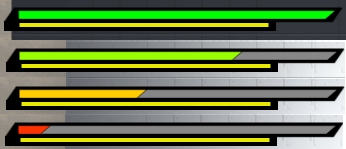
\includegraphics[height=5cm]{images/Lebensleiste.png}
	\caption{Lebensanzeige}
	\label{fig:Lebensanzeige-HUD}
\end{figure}

F"ur das HUD wurde eine Anzeige erstellt, die gleichzeitig auch die Ausdauernd anzeigt. \newline
\begin{lstlisting}[breaklines=true]
//Transform der Lebensleiste
RectTransform healthTransform;
//y-Position der Leiste
float cachedY;
float maxXPos;
float minXPos;
//aktuelle Lebenspunkte
float currentHealth;
float maxHealth;
float newXPos;
AttributeComponent attComp;
Image visualHealth;
\end{lstlisting}
\newpage
An der Stelle an der die Leiste platziert wurde, wurde eine Maske gesetzt. Die Lebenspunkte des Spielers wurden auf die x-Position des Leiste gemappt.\newline

\begin{lstlisting}[breaklines=true]
//Methode zum mappen der Position und Lebenspunkte
private float MapValues(float x, float inMin, float inMax, float outMin, float outMax)
{
	return (x - inMin) * (outMax - outMin) / (inMax - inMin) + outMin;
}

void Update () {
if (currentHealth != attComp.getHealth())
	{
		currentHealth = attComp.getHealth();
		newXPos = MapValues(currentHealth, 0, maxHealth, minXPos, maxXPos);
		healthTransform.localPosition = new Vector3(newXPos, cachedY);
	}
}
\end{lstlisting}
Umso mehr Lebenspunkte der Spieler verliert umso weiter wird die Leiste nach links geschoben. Dank der Maske wird der Teil der Leiste, der "uber sie hinausragt, nicht weiter angezeigt. \newline
\newline Auch wird die Farbe der Leiste zwischen Gr"un und Rot interpoliert, wie in Abbildung 12.1 zu sehen ist.

\begin{lstlisting}[breaklines=true]
if(currentHealth > maxHealth/2)
	{
		visualHealth.color = new Color32((byte)MapValues(currentHealth, maxHealth / 2, maxHealth, 255, 0), 255, 0, 255);
	}

else
	{
		visualHealth.color = new Color32(255, (byte)MapValues(currentHealth, 0, maxHealth / 2, 0, 255), 0, 255);
	}

\end{lstlisting}

F"ur die Ausdaueranzeige wurde ein eigenes Skript geschrieben, welches auf der selben Fuktionsweise basiert, wie die Lebensanzeige, mit dem Unterschied, dass diese sich "uber Zeit von alleine auff"ullt. 
\newpage
\section{Munitionsanzeige}
Auf Tastendruck l"asst sich die Munitionsart des Spielers wechseln. Um dies grafisch zu verdeutlichen wurde am linken unteren Rand ein Panel erstellt, das die Standardmunition beziehungsweise Plasmamunition anzeigt. 
\begin{figure}
	\centering
	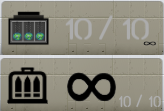
\includegraphics[height=5cm]{images/Munitionsanzeige.png}
	\caption{Munitionsanzeige}
	\label{fig:Munitionsanzeige-HUD}
\end{figure}

\section{Skill-Icons}
Um Abklingzeiten einzuf"uhren und dem Spieler einen Indikator daf"ur zu geben, wie lange er warten muss, bis sich die gew"unschte F"ahigkeit wieder einsetzen zu k"onnen, wurden neben der Munitionsanzeige Icons platziert, die stellvertretend f"ur F"ahigkeiten stehen. Sobald eine F"ahigkeit durch Tastendruck eingesetzt wird, wird das Symbol ausgegraut und die Sekunden bis Freischaltung der F"ahigkeit angezeigt. 
\begin{figure}
	\centering
	
\includegraphics[height=2cm]{images/Skillicons.png}
	\caption{Skill-Icons}
	\label{fig:Skill-Icons-HUD}
\end{figure}